\iffalse
\begin{table*}[thbp]
	\centering
	\scalebox{0.9}{
	\begin{tabularx}{1.1\textwidth}{l|X}
		\hline
		$T$ = Scatter([($M_i$, $R_i$)]) & Scatter a group of messages $M_i$ to receivers $R_i$ respectively, return timestamp $T$. \\
		\hline
		CompletionCallback($f$($T$, IsDelivered, IsFast)) & Register callback $f$ to notify whether a sent scattering $T$ is delivered or discarded, and whether it is an one-RTT fast delivery. \\
		\hline
		$T, M$ = TentativeRecv() & Receive a message $M$ and its timestamp $T$ in order, but may be recalled. \\
		\hline
		RecallCallback($f$($T, M$)) & Register callback $f$ to recall a tentatively received message $M$ at timestamp $T$. \\
		\hline
		$T, M$ = ReliableRecv() & Receive a message $M$ and its timestamp $T$ reliably in order. \\
		\hline
		\hline
		ID = Init(IsHostOrSwitch) & Initialize \sys and get a node ID. \\
		\hline
		Connect(NeighborID) & Connect to a neighbor node (switch or host). \\
		\hline
		Disconnect(NeighborID) & Disconnect from a neighbor node (switch or host). \\
		\hline
		FailureCallback($f$(NodeID, $T$)) & Register callback $f$ for failure notification of node ID at timestamp $T$. \\
		\hline
		NewID = Recover(OldID) & Get a new ID after failure recovery. \\
		\hline
		[$T_i, M_i$] = RedoRecv($T$) & Redo reliable receive since timestamp $T$. \\
		\hline
		DiscardLog($T$) & Discard redo log until timestamp $T$. \\
		\hline
	\end{tabularx}
	}
	\caption{\sys API.}
	\vspace{-25pt}
	\label{tab:api}
\end{table*}
\fi

\begin{figure*}[t!]
	\centering
	\subfloat[Reconfigurable switching chips.\label{fig:p4}]
	{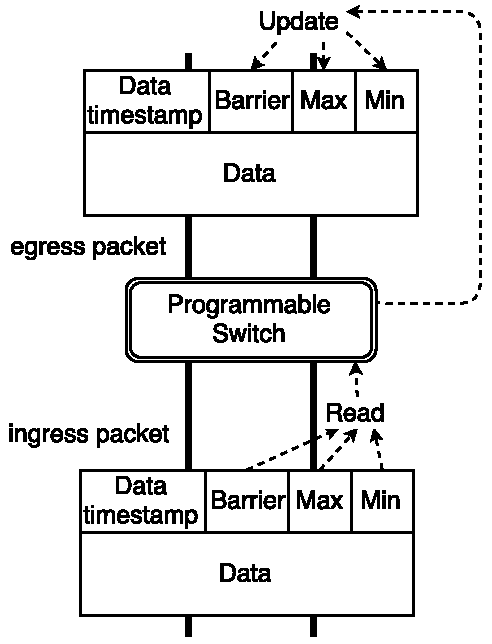
\includegraphics[width=.30\textwidth]{images/p4_implementation.pdf}}
	\hspace{0.04\textwidth}
	\subfloat[Switch CPU.\label{fig:commodity}]
	{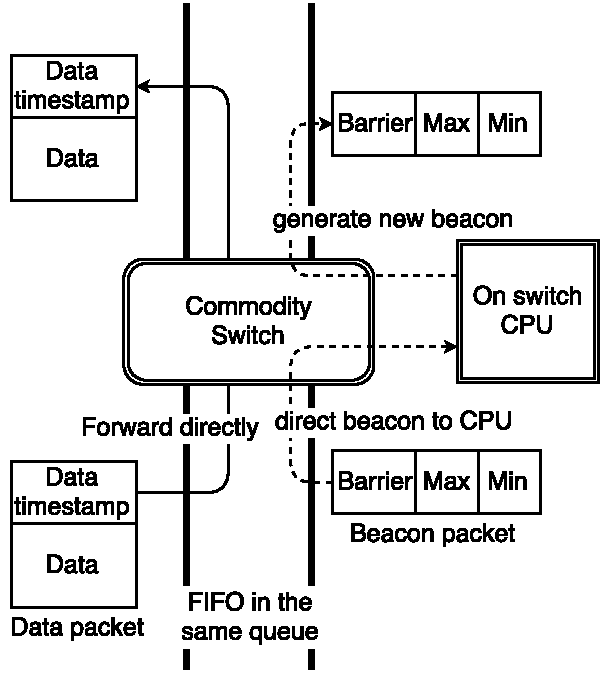
\includegraphics[width=.26\textwidth]{images/commodity_implementation.pdf}}
	\hspace{0.04\textwidth}
	\subfloat[End hosts only.\label{fig:end-host}]
	{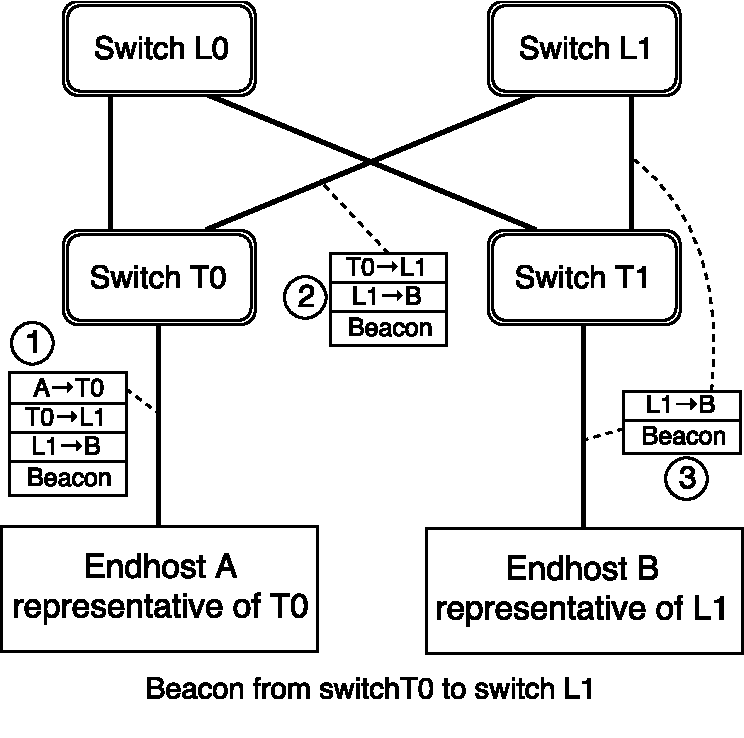
\includegraphics[width=.3\textwidth]{images/endhostonly_implementation.pdf}}
	\vspace{-10pt}
	\caption{\sys dataflow in networks with different programming capabilities.}
	\label{fig:impl}
	\vspace{-10pt}
\end{figure*}


\section{Implementation}
\label{sec:impl}

%\sys{} is implemented on both end hosts and network switches.

%At the end host, \sys requires a reliable transport. The transport can be built over any at-most-once packet transmission interfaces, \textit{e.g.}, UDP, UNIX raw socket, RDMA unreliable datagram~\cite{infinibandrocev2} or netmap~\cite{rizzo2012netmap}. We implement the message transport on the top of a user-mode TCP stack~\cite{dunkels2001design} for loss recovery and congestion control. Beacon packets are sent directly, bypassing the TCP stack. To ensure that retransmitted packets do not violate timestamp monotonicity, we add a TCP option to mark them. In addition, we maintain a mapping from TCP sequence numbers to timestamps, and update commit barrier when a TCP ACK is received.


\subsection{Processing on End Hosts}

We implement an \sys{} library, \texttt{lib1pipe}, at the end host. The library is built on top of RDMA verbs API.
For best effort \sys{}, to ensure timestamp monotonicity, the transport must not retransmit packets.
So, we use RDMA Unreliable Datagram (UD).
Each \sys{} message is sent as one or more UD packets, where \sys{} messages larger than MTU are fragmented into multiple UD packets.
A UD packet has 20 bytes of headers: three timestamps including message, barrier, and commit barrier\footnote{Barriers for best effort and reliable \sys{} are independent. If a cluster only needs one service, only one barrier is needed.}, and a packet sequence number for fast loss detection and defragmentation.
A timestamp is a 48-bit integer, indicating the number of nanoseconds passed on the host. %Since the timestamps wrap around in 4 seconds, 
We use PAWS~\cite{jacobson1992tcp} to handle the timestamp wrap around.
Ideally, we would like to attach timestamps to packets using a programmable NIC.
However, with a standard RDMA NIC, \sys{} assigns timestamp in software.
\sys{} uses PFC~\cite{pfc} to avoid congestion loss. We leave congestion control to future work.

For reliable \sys{}, we use RDMA Reliable Connection (RC) to send messages in prepare phase, and use UD to send commit barrier to ToR switch.
An RC message has 6 bytes of header, representing the timestamp.
The UD message has the same format as best effort \sys{}.
We maintain a receive buffer to reorder messages before delivery and a send buffer to track unACKed messages.

\texttt{lib1pipe} spawns a polling thread to: (1) generate periodic beacon packets; (2) poll RDMA completion queues and process received packets, including generating end-to-end ACKs and retransmitting lost packets; (3) reorder messages in receive buffer, and deliver messages to application threads.
\texttt{lib1pipe} uses polling rather than interrupt because RDMA latency is only $1\sim2 \mu$s, while interrupt would add $\sim10 \mu$s of delay~\cite{yang2012poll}.

All processes on a host connect to the network via RDMA NIC. If the NIC capable of aggregating timestamp barriers, we consider the NIC as a last-level ``switch'' that interconnects processes. Otherwise, processes within a host need to be exposed directly to its Top-of-Rack (ToR) switch, and the ToR aggregates timestamps of all processes in the rack.

The controller is a replicated etcd~\cite{etcd} service.

%We do not need to take special care of intra-host communication between processes: because the packets loopback at the NIC, they take a shorter path than looping back at the switch, so, the packets must arrive earlier than the barrier timestamp.

\iffalse
\subsection{ROMS API on Hosts}
\label{sec:api}

An application uses ROMS via API in Table~\ref{tab:api}.
We implement a ROMS library at the end host. The library is built on top of a user-mode TCP stack~\cite{libvma,dunkels2001design} for loss recovery and congestion control. Beacon packets are sent directly, bypassing the TCP stack. To ensure that retransmitted packets do not violate timestamp monotonicity, we add a TCP option to mark them. In addition, we maintain a mapping from TCP sequence numbers to timestamps, and update delivery barrier when a TCP ACK is received.

We show an example ROMS application: externally consistent~\cite{corbett2013spanner} transactional key-value store (KVS).
The KVS is partitioned to shards according to hash of key, so clients can locate the shard for each key~\cite{nishtala2013scaling,eris}.
Each shard is replicated on multiple hosts.
An independent transaction is initiated by a client host and atomically executes independent GET or PUT operations on multiple keys, which may involve several shards and all replicas in the shards.
%With ROMS, we do not need a centralized transaction manager.
The client scatters the operations to involved shards directly using ROMS \emph{Scatter} API.
If an operation is read-only, it is scattered to one replica of the shard. Otherwise, it is scattered to all replicas of the shard.
To reduce normal case latency, each replica receives operations via \emph{TentativeRecv}, executes them and respond to clients.
However, the replica should be ready to recall tentatively received messages and the client would hold the response until \emph{CompletionCallback}.
If a scattering fails, \emph{RecallCallback} notifies all replicas.
Because removing an operation may affect the results of future operations, each replica re-executes operations since the failed scattering, and respond to clients with a redo mark.
At the same time, \emph{CompletionCallback} notifies the client. Then the client can remove the failed replica and issue a new scattering with a new timestamp.
If a scattering succeeds, the shards confirm the tentatively received messages via \emph{ReliableRecv}, log updated KVs along with timestamp and call \emph{DiscardLog}.
At the same time, \emph{CompletionCallback} notifies the client and tells whether it is an one-RTT fast delivery.
For fast delivery, the client collects responses from all involved shards and replicas.
Otherwise, \emph{i.e.}, packet loss or failure occur, the client waits for responses from all involved shards and replicas with redo mark.

To enable failure recovery, ROMS library logs received messages until \emph{DiscardLog} is called.
When a shard recovers from failure, we replay the KV log and get the last update timestamp, then redo missing operations via \emph{RedoRecv} since the timestamp.
When a client recovers from failure, the uncompleted scatterings are already discarded.
The client may simply report failures to user or implement logging to retry failed scatterings.
\fi


\subsection{In-Network Processing}
\label{sec:in-network-processing}

In the following, we present implementations of in-network processing at three types of network switches with different programming capabilities.


\subsubsection{Reconfigurable Switching Chips}
\label{sec:p4}
A reconfigurable switching chip can maintain 
a handful of states $\mathcal{S}$ and process each packet $P$ through the state machine $P', \mathcal{S}' = f(P, \mathcal{S})$. Hence, we can implement the in-network processing on the reconfigurable chip. 

We implement the in-network processing using P4~\cite{bosshart2014p4} and compile it to Barefoot Tofino~\cite{tofino}. \sys{} needs 2 state registers \emph{per input link}, storing the two barriers for best effort and reliable \sys{}, respectively. \sys{} also needs 2 state registers to store the minimum of per-link barriers. As Figure~\ref{fig:p4} shows, for each packet, barrier of the input link is first updated, then switch barrier is updated to the minimum of link barrier and the original switch barrier. Finally, the barrier in packet is updated to the switch barrier. The control plane software routinely checks link barriers, and report failure if a barrier significantly lags behind.


%We implement the in-network processing using P4~\cite{bosshart2014p4} and compile it to Barefoot Tofino~\cite{tofino}. \sys needs 8 state registers per input link and 5 state registers per output link. Each data packet carries three timestamp fields: message timestamp, loss-free barrier and delivery barrier, as well as loss encountered flag (Algorithm~\ref{alg:loss-detection}).
%A timestamp is a 6-byte integer, indicating the number of nanoseconds passed on the host. %Since the timestamps wrap around in 7.8 hours, 
%We use PAWS~\cite{jacobson1992tcp} to handle the timestamp wrap around.
%%to compare timestamps: If $s$ and $t$ are timestamps, $s < t$ if and only if $0 < t - s < 2^{47}$, computed in 48-bit unsigned arithmetic. 
%As shown in Figure~\ref{fig:p4}, the beacon packets carries not only the same set of timestamps and flag as data packets, but also information for minimax clock synchronization.
%% (Algorithm~\ref{alg:minimax}).

\subsubsection{Switch CPU}
\label{sec:commodity}

For a switch without a reconfigurable router chip, \textit{e.g.,} Arista 7060CX, we implement in-network processing on the switch CPU.
%Data-plane programmable switches are currently not widely available in data centers.
Although commodity switches cannot process packets in data plane, they have a CPU to process control-plane packets, analogous to directly connecting a server to a port of the switch.
Compared to server CPUs and NICs, the switch CPU is typically less powerful (\textit{e.g.}, 4 cores at 1~GHz) and has lower bandwidth (\textit{e.g.}, 1 Gbps).

Because the switch CPU cannot process every packet, data packets are forwarded by the switching chip directly, as Figure~\ref{fig:commodity} shows.
The switch CPU sends beacons periodically on each output link, regardless of whether the link is idle or busy.
Because data and beacon packets are FIFO in switch queues and on network links, the barrier property is preserved. On receivers, buffered data packets are delivered to the application according to barriers in beacon packets.

Compared with the reconfigurable switching chip, this approach slacks the barriers in two aspects.
First, the barriers are updated by periodical beacons instead of by every packet.
Second, compared to switching chip, switch CPU introduces higher processing delay.
So, the average delay overhead is (switch processing delay $\times$ number of hops + beacon interval/2 + clock skew).

\subsubsection{Delegate Switch Processing to a Host}
\label{sec:end-host}

If the switch vendor does not expose access interfaces to switch CPUs, we can offload the beacon processing to end hosts. The challenge is to maintain the FIFO property on network links, \emph{i.e.}, beacons with barrier timestamps on a network link $L$ must pass through $L$. To this end, we designate an \emph{end-host representative} for each network switch. %The location of the representative is arbitrary and does not need to be unique.

As Figure~\ref{fig:end-host} shows, for two directly connected switches $S_1, S_2$ and their representatives $H_1, H_2$, beacon packets from $H_1$ to $H_2$ need to go through the link $S_1 \rightarrow S_2$. If the route between two representatives does not go through $S_1 \rightarrow S_2$, beacon packets needs to detour: they are sent with three layers of IP headers: $H_1 \rightarrow S_1$, $S_1 \rightarrow S_2$, and $S_2 \rightarrow H_2$.
We install tunnel termination rules in each network switch to de-capsulate one layer of IP header, so the beacon packet will traverse through $H_1 \rightarrow S_1 \rightarrow S_2 \rightarrow H_2$.

Beacon packets use one-sided RDMA write to update per-input-link barriers on representative host. A thread on the host iteratively computes minimum barrier and broadcasts new beacons to representatives of downstream switches.
The average delay overhead is ((RTT between switch and host + host processing delay) $\times$ number of hops + beacon interval/2 + clock skew). Because end hosts support RDMA and its CPUs are more powerful than switch's, the overall reordering delay may be shorter than using switch CPU.

%\textbf{Note:} reliable \sys{} does not rely on the best effort barrier. If a cluster only needs reliable \sys{} service, only one commit barrier needs to be maintained. If both best effort and reliable \sys{} are needed, switches need to maintain two barriers independently.
